\begin{flushright} {\tiny {\color{gray} basis\_p2\_2D.tex}} \end{flushright}
%~~~~~~~~~~~~~~~~~~~~~~~~~~~~~~~~~~~~~~~~~~~~~~~~~~~~~~~~~~~~~~~~~~~~~~~~~~~~~~~~~~~~~~~~~~~~~~~~~~

\begin{flushright} {\tiny {\color{gray} (tikz\_P2.tex)}} \end{flushright}
%~~~~~~~~~~~~~~~~~~~~~~~~~~~~~~~~~~~~~~~~~~~~~~~~~~~~~~~~~~~~~~~~~~~~~~~~~~~~~~~~~~~~~~~~~~~~~~~~~~

\begin{center}
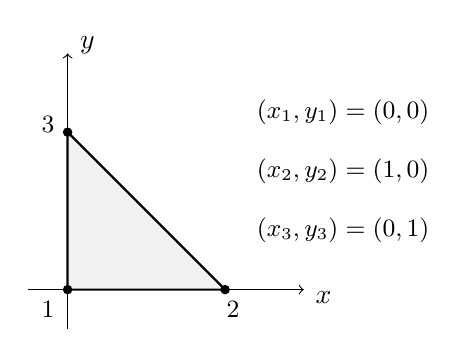
\begin{tikzpicture}
%\draw[step=0.5cm,gray,very thin] (0,0) grid (4,4); 
\draw[fill=gray!10,gray!10] (0.5,0.5)--(2.5,0.5)--(0.5,2.5)--cycle;
\draw[thick] (0.5,0.5)--(2.5,0.5)--(0.5,2.5)--cycle;
\draw [->] (0,0.5) -- (3.5,0.5);
\draw [->] (0.5,0) -- (0.5,3.5);
\node[] at (3.75,0.4) {$x$};
\node[] at (0.75,3.6) {$y$};
\draw[black,fill=black] (0.5,0.5)   circle (1.5pt);
\draw[black,fill=black] (2.5,0.5)   circle (1.5pt);
\draw[black,fill=black] (0.5,2.5)   circle (1.5pt);
\node[] at (0.25,0.25) {\small $1$};
\node[] at (2.6,0.25) {\small $2$};
\node[] at (0.25,2.6) {\small $3$};
\node[] at (4,2.75) {\small $(x_1,y_1)=(0,0)$};
\node[] at (4,2) {\small $(x_2,y_2)=(1,0)$};
\node[] at (4,1.25) {\small $(x_3,y_3)=(0,1)$};
\end{tikzpicture}
\end{center}



The basis polynomial is then
\[
f(r,s) = c_1 + c_2 r + c_3 s + c_4  r^2 + c_5 rs  + c_6 s^2
\]
We have 
\begin{eqnarray}
f_1 = f(r_1,s_1) &=& c_1 \nonumber\\
f_2 = f(r_2,s_2) &=& c_1 + c_2 + c_4\nonumber\\
f_3 = f(r_3,s_3) &=& c_1 + c_3 + c_6\nonumber\\
f_4 = f(r_4,s_4) &=& c_1 + c_2/2 + c_4/4\nonumber\\
f_5 = f(r_5,s_5) &=& c_1 + c_2/2 + c_3/2  + c_4/4 + c_5/4 + c_6/4\nonumber\\
f_6 = f(r_6,s_6) &=& c_1 + c_3/2 + c_6/4\nonumber
\end{eqnarray}
This can be cast as $\vec{f}={\bm A}\cdot \vec{c}$ where ${\bm A}$ is a $6\times6$ matrix:
\[
{\bm A}=
\left(
\begin{array}{cccccc}
1&0   &  0  & 0   & 0   & 0\\
1&1   &  0  & 1   & 0   & 0\\
1&0   &  1  & 0   & 0   & 1\\
1&1/2 &  0  & 1/4 & 0   & 0\\
1&1/2 &  1/2& 1/4 & 1/4 & 1/4\\
1&0   &  1/2& 0   & 0   & 1/4
\end{array}
\right)
\]
As it turns out it is rather trivial to compute the inverse of this matrix:
\[
{\bm A}^{-1}=
\left(
\begin{array}{cccccc}
1  & 0 & 0  & 0  & 0 & 0  \\
-3 & -1& 0  & 4  & 0 & 0 \\
-3 & 0 & -1 & 0  & 0 & 4 \\
2  & 2 & 0  & -4 & 0 & 0  \\
4  & 0 & 0  & -4 & 4 & -4 \\
2  & 0 & 2  & 0  & 0 & -4
\end{array}
\right)
\]
Using $\vec{c}={\bm A}^{-1}\cdot \vec{f}$ one then obtains:
\begin{eqnarray}
c_1 &=& f_1 \nn\\
c_2 &=& -3f_1-f_2+4f_4\nn\\
c_3 &=& -3f_1-f_3+4f_6  \nn\\
c_4 &=& 2f_1+2f_2-4f_4 \nn\\
c_5 &=& 4f_1-4f_4+4f_5-4f_6 \nn\\
c_6 &=& (2f_1+2f_3-4f_6 \nn
\end{eqnarray}
and then
\begin{eqnarray}
f(r,s) 
&=& f_1 + (-3f_1-f_2+4f_4) r + (-3f_1-f_3+4f_6)s \nonumber\\
&& +(2f_1+2f_2-4f_4)r^2 + (4f_1-4f_4+4f_5-4f_6) rs + (2f_1+2f_3-4f_6)s^2 \nonumber\\
&=& \sum_{i=1}^6 \bN_i(r,s) f_i
\end{eqnarray}
with
\begin{mdframed}[backgroundcolor=blue!5]
\begin{eqnarray}
\bN_1(r,s) &=& 1-3r-3s+2r^2+4rs+2s^2 \nonumber\\
\bN_2(r,s) &=& -r+2r^2 \nonumber\\
\bN_3(r,s) &=& -s+2s^2 \nonumber\\
\bN_4(r,s) &=& 4r-4r^2-4rs \nonumber\\
\bN_5(r,s) &=& 4rs \nonumber\\
\bN_6(r,s) &=& 4s-4rs-4s^2 \nonumber
\end{eqnarray}
\end{mdframed}

The derivatives are as follows:
\begin{eqnarray}
\frac{\partial \bN_1}{\partial r}(r,s) &=&  -3+4r+4s \nn\\ 
\frac{\partial \bN_2}{\partial r}(r,s) &=&  -1+4r\nn\\ 
\frac{\partial \bN_3}{\partial r}(r,s) &=&  0\nn\\ 
\frac{\partial \bN_4}{\partial r}(r,s) &=&  4-8r-4s\nn\\ 
\frac{\partial \bN_5}{\partial r}(r,s) &=&  4s\nn\\ 
\frac{\partial \bN_6}{\partial r}(r,s) &=&  -4s\nn
\end{eqnarray}

\begin{eqnarray}
\frac{\partial \bN_1}{\partial s}(r,s) &=&  -3+4r+4s\nn\\ 
\frac{\partial \bN_2}{\partial s}(r,s) &=&  0\nn\\ 
\frac{\partial \bN_3}{\partial s}(r,s) &=&  -1+4s\nn\\ 
\frac{\partial \bN_4}{\partial s}(r,s) &=&  -4r\nn\\ 
\frac{\partial \bN_5}{\partial s}(r,s) &=&  4r\nn\\ 
\frac{\partial \bN_6}{\partial s}(r,s) &=&  4-4r-8s\nn
\end{eqnarray}
